\documentclass[tikz, border=0.2mm]{standalone}
\usepackage{amsmath,xparse}
\ExplSyntaxOn
% 1. Create a variable to hold the path construction
\tl_new:N \l_lattice_path_tl
% 2. Define the main command
\NewDocumentCommand{\latticePath}{ O{} m m }
 {
  % Clear the variable for the new path
  \tl_clear:N \l_lattice_path_tl
  % Loop through the input string (#3)
  \str_map_inline:nn { #3 }
   {
    % Append the TikZ code to the variable based on the character
    \str_case:nnF { ##1 }
     {
       % Numpad
       {1}{ \tl_put_right:Nn \l_lattice_path_tl { --~++(-1,-1) } } % SW
       {2}{ \tl_put_right:Nn \l_lattice_path_tl { --~++(0,-1)  } } % S
       {3}{ \tl_put_right:Nn \l_lattice_path_tl { --~++(1,-1)  } } % SE
       {4}{ \tl_put_right:Nn \l_lattice_path_tl { --~++(-1,0)  } } % W
       {6}{ \tl_put_right:Nn \l_lattice_path_tl { --~++(1,0)   } } % E
       {7}{ \tl_put_right:Nn \l_lattice_path_tl { --~++(-1,1)  } } % NW
       {8}{ \tl_put_right:Nn \l_lattice_path_tl { --~++(0,1)   } } % N
       {9}{ \tl_put_right:Nn \l_lattice_path_tl { --~++(1,1)   } } % NE
       % Cardinals
       {n}{ \tl_put_right:Nn \l_lattice_path_tl { --~++(0,1)   } }
       {s}{ \tl_put_right:Nn \l_lattice_path_tl { --~++(0,-1)  } }
       {e}{ \tl_put_right:Nn \l_lattice_path_tl { --~++(1,0)   } }
       {w}{ \tl_put_right:Nn \l_lattice_path_tl { --~++(-1,0)  } }
       % Relatives
       {u}{ \tl_put_right:Nn \l_lattice_path_tl { --~++(0,1)   } }
       {d}{ \tl_put_right:Nn \l_lattice_path_tl { --~++(0,-1)  } }
       {l}{ \tl_put_right:Nn \l_lattice_path_tl { --~++(-1,0)  } }
       {r}{ \tl_put_right:Nn \l_lattice_path_tl { --~++(1,0)   } }
     }
     {
       % Fallback (ignore unknown characters)
     }
   }
   % 3. Execute the Draw Command using the constructed path
   % Note: We use ~ for spaces inside ExplSyntax
   \draw[line~width=4.0pt, line~cap=round, line~join=round, #1] (#2) \l_lattice_path_tl ;
 }
\ExplSyntaxOff


\begin{document}
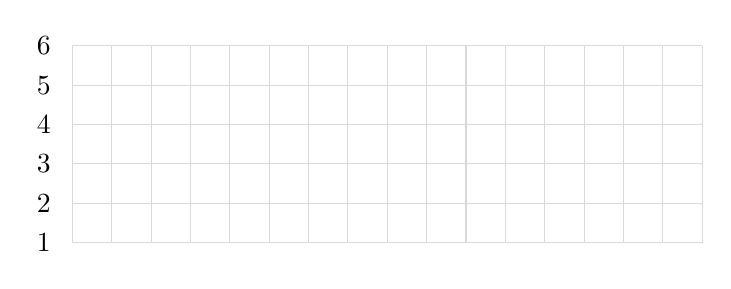
\begin{tikzpicture}[scale=0.5]
    % Draw grid
    \draw[gray!30, thin] (0,1) grid (16,6);

    % Draw axis numbers
    \foreach \y in {1,...,6}
        \node[left] at (-0.3,\y) {\y};

    \latticePath{0,1}{nnnnne}
    \latticePath{1,1}{nnnenene}
    \latticePath{2,1}{nenenenne}
    \latticePath{3,1}{eennenneene}
    \latticePath{6,1}{neneneenenee}
    \latticePath{7,1}{eneeneneneen}
    \latticePath{9,1}{eeneenenenne}
\end{tikzpicture}
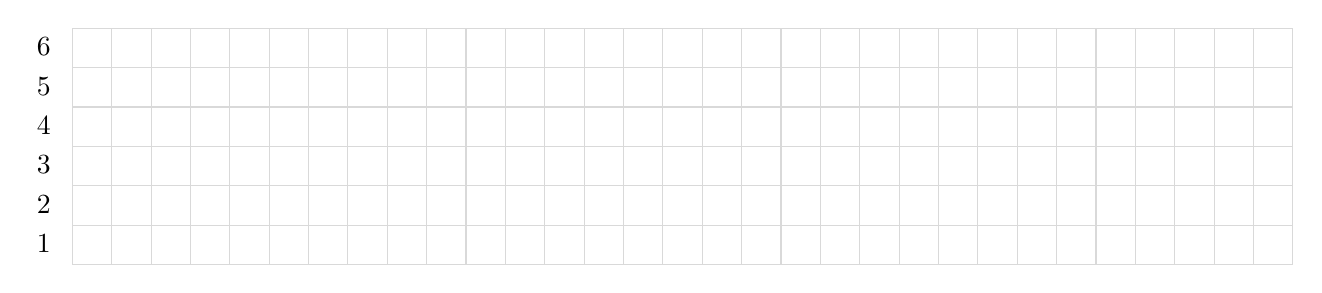
\begin{tikzpicture}[scale=0.5]
    % Draw grid
    \draw[gray!30] (0,1) grid (31,7);

    % Draw axis numbers
    \begin{scope}[yshift=1.5em]
    \foreach \y in {1,...,6}
        \node[left] at (-0.3,\y) {\y};
    \end{scope}

    \latticePath{ 2,1}{779797}
    \latticePath{ 4,1}{797979}
    \latticePath{10,1}{777797}
    \latticePath{14,1}{777977}
    \latticePath{16,1}{779779}
    \latticePath{18,1}{977797}
    \latticePath{20,1}{979779}
    \latticePath{22,1}{997977}
    \latticePath{24,1}{999777}
    \latticePath{26,1}{999997}
\end{tikzpicture}


\end{document}
